
\documentclass[final]{beamer}

\usepackage[scale=1.24]{beamerposter} % Use the beamerposter package for laying out the poster

\usetheme{confposter} % Use the confposter theme supplied with this template

\setbeamercolor{block title}{fg=nblue, bg=white} % Colors of the block titles
\setbeamercolor{block body}{fg=black, bg=white} % Colors of the body of blocks
\setbeamercolor{block alerted title}{fg=white, bg=dblue!70} % Colors of the highlighted block titles
\setbeamercolor{block alerted body}{fg=black, bg=dblue!10} % Colors of the body of highlighted blocks
% Many more colors are available for use in beamerthemeconfposter.sty
\setbeamercolor{itemize item}{fg=nblue, bg=white}%-----------------------------------------------------------
% Define the column widths and overall poster size
% To set effective sepwid, onecolwid and twocolwid values, first choose how many columns you want and how much separation you want between columns
% In this template, the separation width chosen is 0.024 of the paper width and a 4-column layout
% onecolwid should therefore be (1-(# of columns+1)*sepwid)/# of columns e.g. (1-(4+1)*0.024)/4 = 0.22
% Set twocolwid to be (2*onecolwid)+sepwid = 0.464
% Set threecolwid to be (3*onecolwid)+2*sepwid = 0.708

\newlength{\sepwid}
\newlength{\onecolwid}
\newlength{\twocolwid}
\newlength{\threecolwid}
\setlength{\paperwidth}{48in} % A0 width: 46.8in
\setlength{\paperheight}{36in} % A0 height: 33.1in
\setlength{\sepwid}{0.024\paperwidth} % Separation width (white space) between columns
\setlength{\onecolwid}{0.30\paperwidth} % Width of one column
\setlength{\topmargin}{-0.5in} % Reduce the top margin size
%-----------------------------------------------------------

\usepackage{graphicx}  % Required for including images
\usepackage{wrapfig}
\usepackage{lipsum}
\usepackage{booktabs} % Top and bottom rules for tables


\usepackage{calrsfs}
\usepackage{amsmath}
\DeclareMathOperator*{\argmax}{argmax}
\DeclareMathOperator*{\argmin}{argmin}
\DeclareMathAlphabet{\pazocal}{OMS}{zplm}{m}{n}
\newcommand{\La}{\mathcal{L}}
\newcommand{\Lb}{\pazocal{L}}

\usepackage{tcolorbox}

%----------------------------------------------------------------------------------------
%	TITLE SECTION 
%----------------------------------------------------------------------------------------

\title{Sentiment Analysis for Amazon Musical Instruments Reviews} % Poster title

\author{Eduard Mihranyan} % Author(s)


%----------------------------------------------------------------------------------------

\begin{document}

\addtobeamertemplate{block end}{}{\vspace*{2ex}} % White space under blocks
\addtobeamertemplate{block alerted end}{}{\vspace*{2ex}} % White space under highlighted (alert) blocks

\setlength{\belowcaptionskip}{2ex} % White space under figures
\setlength\belowdisplayshortskip{2ex} % White space under equations

\begin{frame}[t] % The whole poster is enclosed in one beamer frame

\begin{columns}[t] % The whole poster consists of three major columns, the second of which is split into two columns twice - the [t] option aligns each column's content to the top

\begin{column}{\sepwid}\end{column} % Empty spacer column

\begin{column}{\onecolwid} % The first column

%----------------------------------------------------------------------------------------
%	OBJECTIVES
%----------------------------------------------------------------------------------------

\begin{block}{Introduction}
\begin{itemize}
\item Sentiment analysis of product reviews, an application problem, has recently become very popular in text mining and computational linguistics research.
\item Here, we want to study the correlation between the Amazon musical instruments reviews and the rating given by the customers
\item The objective of this paper is to classify the positive and negative reviews of the customers over different products and build a supervised learning model to polarize large amounts of reviews.

\end{itemize}
\end{block}


\begin{block}{Dataset}
\begin{itemize}


\item Our dataset comes from Kaggle. It is Amazon Musical Instruments Reviews. There are 10,261 rows in total. Each row consists of a review followed by a rate, which is an integer from 1 to 5. The distributions of the rates are shown in the figure below. 

\begin{figure}
\raggedright
	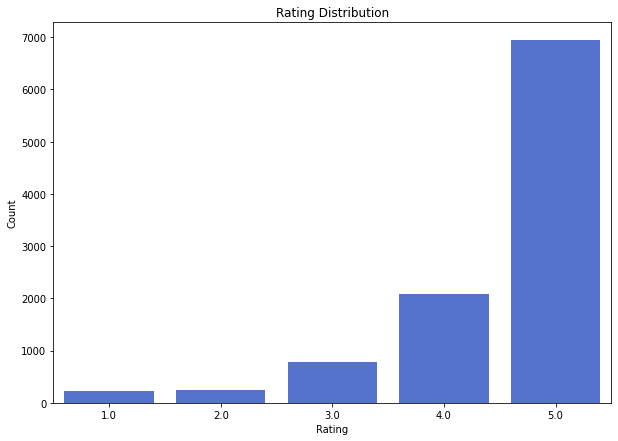
\includegraphics[width=0.6\linewidth, height=0.35\textheight, keepaspectratio]{figure1.png}
	\label{fig:feature_imp}
\item As we can see, the distribution of the dataset is super imbalanced, which will be discussed
later. There are rows without rate, which we just treat as missing data
\end{figure}





\end{itemize}
\end{block}

\begin{block}{Features}

\begin{itemize}

\item The features we extracted include two types.
\item We  first  removed  punctuation,then  we  tokentized  the  sentences  in  the  text,   andeventually lemmatized each word to its lemma. We haveused keras Tokenizer and converted texts to sequences. We have also done padding to equalize the lengths of allinput reviews. 
\item Alternatively, we have used standard count vectorization and tf-idf vectorization techniques. We have built also bigrams and trigrams to also capture word combinations. 

\end{itemize}
\end{block}

\end{column} % End of the first column

\begin{column}{\sepwid}\end{column} % Empty spacer column

\begin{column}{\onecolwid} % Begin a column which is two columns wide (column 2)
\begin{block}{Models}
\begin{itemize}
\item Naive Bayes:
This algorithm assumes that $x_i$'s are conditionally independent given $y$.
\[p(x_1,...,x_k|y)=\prod_{i=1}^{k} p(x_i|y)\]


\item Logistic regression:
This algorithm tries to maximimize the following likelihood function:

\[l(\theta)= \sum_{i=1}^{m}y^{(i)}\log h(x^{(i)})+(1-y^{(i)})\log (1-h(x^{(i)}))\]
\item SVM: 
Geometrically given two types of points, circles and xi, in a space, it tries to maximize the minimum distance from one of the points to the other.
\[\argmax_{\gamma,\omega,b}\frac{1}{2}\left\|\omega\right\|^2\]
\[s.t. y^{i}(w^{T}x+b)>=1,i=1,2,...,m\]


\item XGBoost: 
\[\Lb (\phi) = \Sigma_i l(\hat{y}_i, y_i) + \Sigma_k \Omega (f_k) \]
\[where: \Omega (f) = \gamma T + \frac{1}{2}\lambda ||\omega||^2\]

\item LSTM:

\begin{figure}
	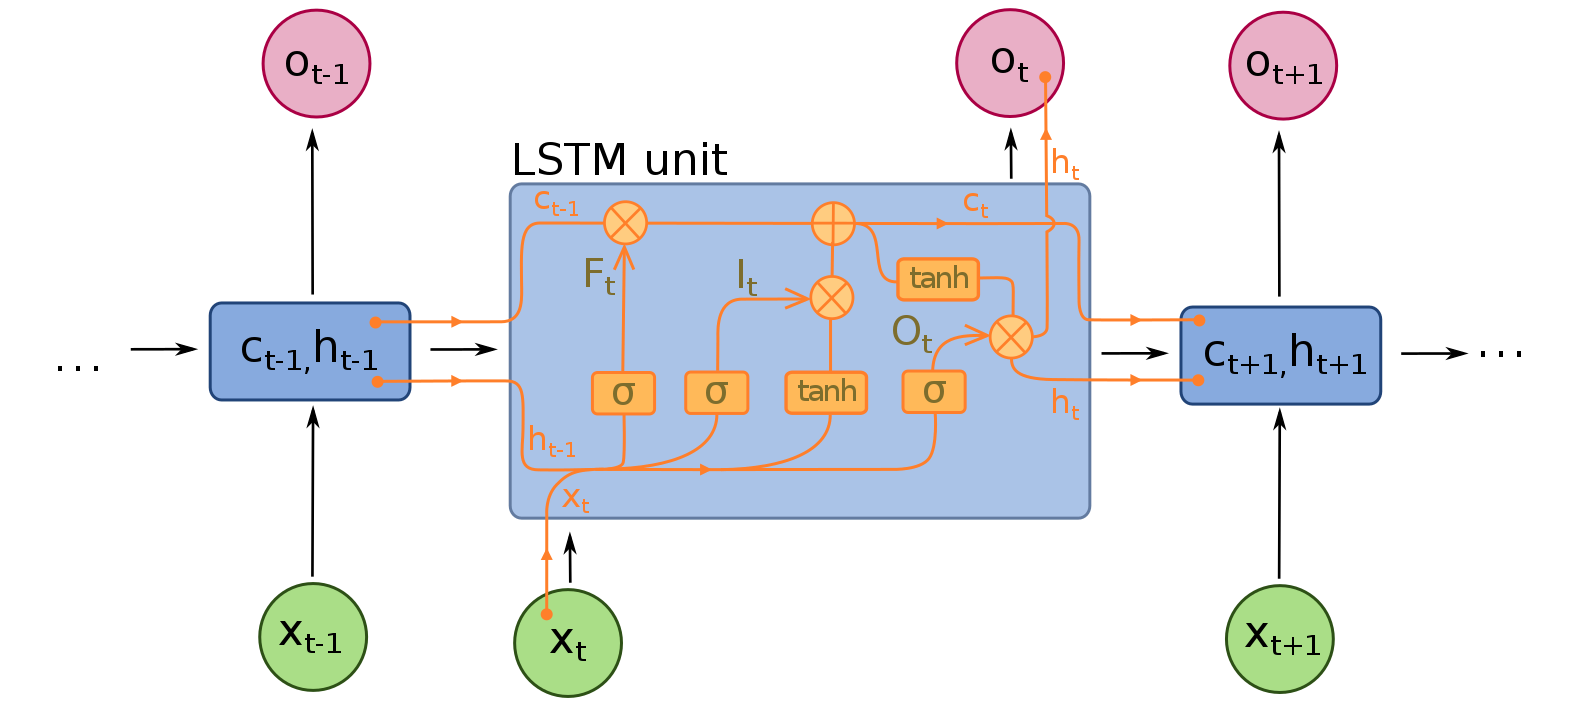
\includegraphics[width=0.3\linewidth, height=0.35\textheight, keepaspectratio]{figure2.png}
	\label{fig:feature_imp}

\end{figure}


A common LSTM unit is composed of a cell, an input gate, an
output gate and a forget gate.

\end{itemize}
\end{block}

\begin{block}{Analysis}

\begin{itemize}
\item The dataset is unbalanced. Based on the result, the model may not have a good generalization of these data. That’s why some of the models have poor accuracy when weight classes or synthetically generate data.
\item One of the methods used for balancing the training data was SMOTE. SMOTE synthetically generates new data points of minority class considering k-nearest neighbors of each point in the class. However, results were not as effective as it was expected. 
\item As the result have shown all models performed best by transforming text to sequences rather than count vectorizing or tf-idf vectorization. 
\end{itemize}


\end{block}
\end{column} % End of the second column

\begin{column}{\sepwid}\end{column} % Empty spacer column

\begin{column}{\onecolwid} % The third column

%\setbeamercolor{block title}{fg=red,bg=white}
\begin{block}{Results}

\begin{itemize}
\item The entire dataset of 10,261 reviews was divided into a training set of size 8208 (80\%)and a test set of size 2053 (20\%).

\item With 2067-d input features representing review text, we implemented Multinomial Naive Bayes, SVM with Linear Kernel, Logistic Regression, XGBoost and LSTM.

\item As we can see from the table of performance LSTM gives significantly higher F1 score and ROC and it's also good in terms of accuracy.

\bigskip
\begin{center}

\begin{tabular}{ l|c|c|c} 

  Models & Accuracy & F1 score & ROC  \\
 \hline
 Multinomial NB & 80.4\% & 0.52 & 0.52  \\ 
 Logistic Regression & 51.7\% & 0.43 & 0.51  \\ 
 Linear SVM & 79.0\% & 0.52 & 0.52 \\ 
 XGBoost & 88.4\% & 0.50 & 0.52 \\ 
 XGBoost+SMOTE & 82.0\% & 0.53 & 0.53 \\ 
 LSTM & 86.8\% & 0.69 & 0.72 \\
 LSTM+SMOTE & 87.3\% & 0.72 & 0.74 \\
 \hline

\end{tabular}

\bigskip
\end{center}
\begin{center}
 \caption{Table1. Performance of different models}
\end{center}

\end{itemize}
\end{block}


\begin{block}{Future Work}
If we have more time, we want to change to another dataset which has a relatively more balanced dataset. The training at the moment is not that satisfactory. We also want to go deeper in the
LSTM neural network in which case we might get better accuracy. 


\end{block}

\begin{block}{References}

\begin{thebibliography}{9}

\bibitem{Dataset}
Dataset Link: \url{https://www.kaggle.com/eswarchandt/amazon-music-reviews}
\bibitem{Dave2003} 
K. Dave, S. Lawrence, and D. M. Pennock. Mining the
peanut gallery: Opinion extraction and semantic classification
of product reviews. In \textit{Proceedings of the 12th international
conference on World Wide Web}, pages 519–528. ACM, 2003..
\bibitem{Lui2012} 
B. Liu and L. Zhang.\textit{A Survey of Opinion Mining and Sentiment Analysis}, pages 415–463. Springer US, Boston, MA,
2012.
\bibitem{Rain2013} 
C. Rain. Sentiment analysis in amazon reviews using probabilistic machine learning. \textit{Swarthmore College}, 2013.
\end{thebibliography}
\end{block}

\end{column} % End of the third column

\end{columns} % End of all the columns in the poster

\end{frame} % End of the enclosing frame

\end{document}
